\documentclass[10pt, compress]{beamer}

\usetheme{m}

\usepackage{booktabs}
\usepackage[scale=2]{ccicons}
\usepackage{minted}

\usepackage{bibentry}
\bibliographystyle{apalike}

\usepgfplotslibrary{dateplot}

\usemintedstyle{trac}

\renewcommand\footnotemark{}
\renewcommand\footnoterule{}

\title{Nucleo-olivary inhibition explains extinction on a computational model of the vestibulo-ocular reflex}
\subtitle{}
\date{July 7, 2015}
\author{Xavier Duran, supervised by Ivan Herreros and Paul Verschure}
\institute{Master in Cognitive Systems and Interactive Media}

\begin{document}

\maketitle

\begin{frame}[fragile]
  \frametitle{Vestibulo-ocular reflex (VOR)}
  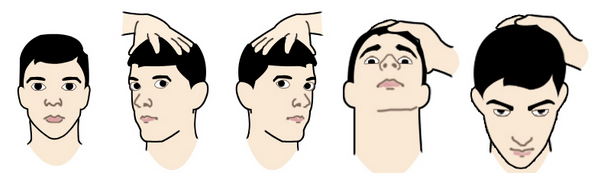
\includegraphics[scale=0.5]{images/vor.png}
  \newline
  \footnote{\url{http://bit.ly/1Ox3Qd6}}
  \newline
  This reflex functions to \textbf{stabilize images} on the retinas during \textbf{head movement} by producing \textbf{eye movements} in the direction opposite to head movement, thus preserving the image on the center of the visual field.
\end{frame}

\begin{frame}[fragile]
  \frametitle{VOR adaptation}
  VOR adaptation is \textbf{trained with light} and \textbf{measured in the dark}
  \cite{Boyden2004}
  \newline
  \newline
  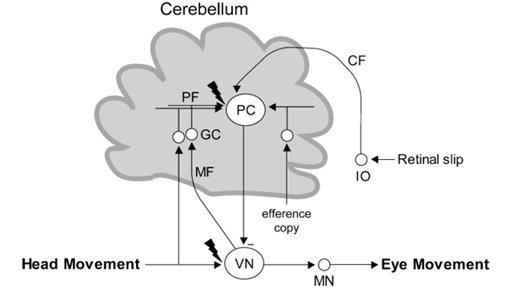
\includegraphics[scale=0.4]{images/boyden.png}
\end{frame}

\begin{frame}[fragile]
  \frametitle{Extinction of the learned adaptation}
  \begin{itemize}
    \item \textbf{head movements} in the absence of \textbf{visual stimulation} cause a loss of the learned \textbf{eye movement response}
    \item changes in the amplitude, or gain of the VOR
    \item is mediated by an \alert{active, extinction-like process} (not by passive forgetting)
  \end{itemize}
  \cite{Cohen2004}
\end{frame}

\begin{frame}[fragile]
  \frametitle{Problem statement}
  \begin{quote}
    State of the art computational models of the vestibulo-ocular reflex don't define a physiological mechanism for extinction
  \end{quote}
\end{frame}

\begin{frame}[fragile]
  \frametitle{Nucleo-olivary inhibition (NOI): a candidate signal}
  Inhibition of climbing fibres (retinal slip) serves as a teaching signal for extinction \cite{Medina2002}
  \begin{figure}
    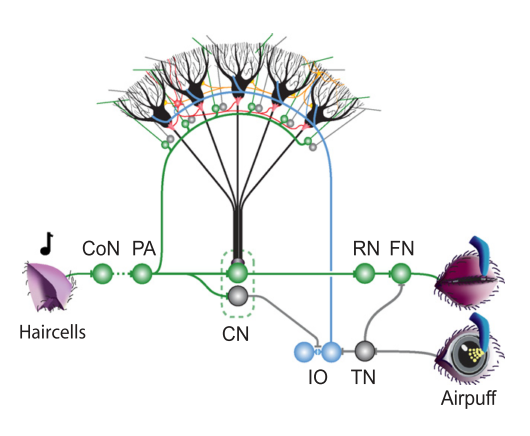
\includegraphics[scale=0.3]{images/schonewille-ebc.png}
    \caption{Neuroanatomical circuitry involved in eyeblink conditioning \cite{Schonewille2010}}
  \end{figure}
\end{frame}

\begin{frame}[fragile]
  \frametitle{Research question}
  \begin{quote}
    \textbf{Would nucleo-olivary inhibition explain extinction in the vestibulo-ocular reflex computational models?}
  \end{quote}
  \begin{block}{\alert{In direct evidence}}
    \begin{itemize}
      \item There is extinction of the adaptive response in the absence of peripheral error
      \item NOI has a role in the eye-blink reflex. The gain of the NOI is what determines the amplitude of the response on adaptive reflexes \cite{Emken2007, Herreros2013b}
      \note{Motor learning in the vestibulo-ocular reflex (VOR) and eyeblink conditioning use similar neural circuitry, and they may use similar cellular plasticity mechanisms.}
    \end{itemize}
  \end{block}
\end{frame}

\begin{frame}[fragile]
  \frametitle{Hypothesis}
  \begin{quote}
    Adding nucleo-olivary inhibition on a vestibulo-ocular reflex computational model would explain extinction as in the experimental behavior of the reflex
  \end{quote}
\end{frame}

\section{Methods}

\begin{frame}[fragile]
  \frametitle{A bottom-up model computational model of the VOR}
  This computational model is made bottom-up from physiological and behavioral observations
  \begin{itemize}
    \item Plasticity on the cerebellar cortex
    \begin{itemize}
      \item quick
      \item short-term
      \item error-based learning
    \end{itemize}
    \item Plasticity on the brainstem
    \begin{itemize}
      \item slow
      \item long-term
    \end{itemize}
  \end{itemize}
  \cite{Clopath2014}
\end{frame}

\begin{frame}[fragile]
  \frametitle{Learning balance}
  \begin{itemize}
    \item learned adaptation at the cerebellar cortex is slowly transfered to the brainstem
    \item cortical plasticity remains flexible to further adaptations
    \item savings help faster response on reacquisition
  \end{itemize}
  \begin{figure}
    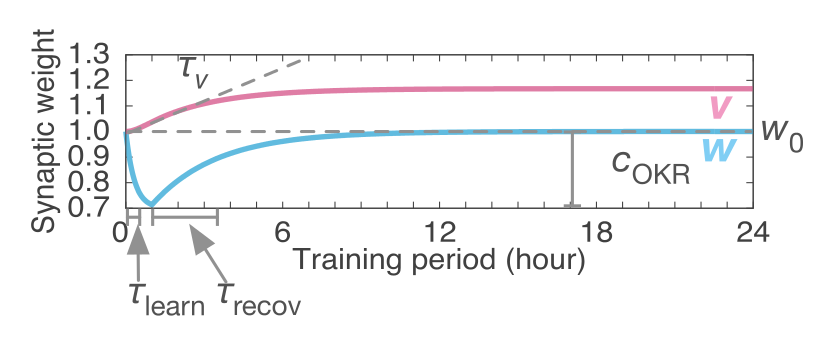
\includegraphics[scale=0.3]{images/okr_memory.png}
    \caption{Short and long-term memory on eyeblink reflex adaptation \cite{Yamazaki2015}}
  \end{figure}
\end{frame}

\begin{frame}[fragile]
  \frametitle{Adding NOI to Clopath's model}
  Extinction on Clopath's model
  \begin{itemize}
    \item Weakly modulated by head movement (vestibular signal)
    \item Weights on cortical plasticity decay linearly to their initial value
  \end{itemize}
  Extinction on NOI model
  \begin{itemize}
    \item \alert{Extinction is defined as proportional to cerebellar output}
    \item More simple mechanism
  \end{itemize}
\end{frame}

\begin{frame}[fragile]
  \frametitle{VOR phase reversal training protocol simulation}
  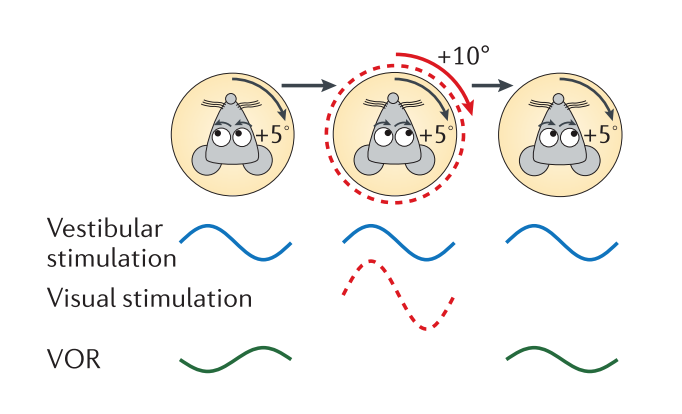
\includegraphics[scale=0.25]{images/vor_adaptation.png}

  \cite{Gao2012a}
  \begin{itemize}
    \item Day 1: VOR cancellation
    \item Day 2: VOR reversal with gain -0.5
    \item Day 3 and 4: Phase reversal with gain -1
    \pause
    \item One week of light deprivation with vestibular stimulation
  \end{itemize}
\end{frame}

\section{Results}

\begin{frame}[fragile]
  \frametitle{Reproducing Clopath's results}
  \begin{columns}[onlytextwidth]
    \column{0.5\textwidth}
      \begin{figure}
        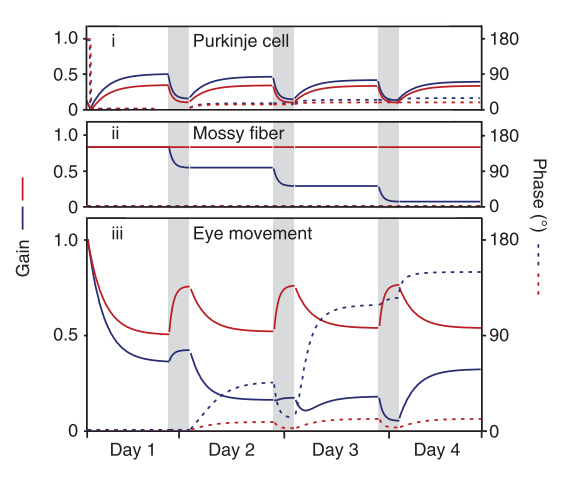
\includegraphics[scale=0.25]{images/gain.png}
        \caption{Experimental results (left) and simulations (right)}
      \end{figure}
    \column{0.5\textwidth}
    \begin{figure}
      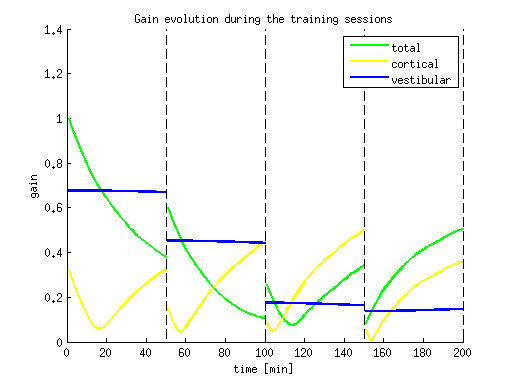
\includegraphics[scale=0.35]{images/longnoi_12.png}
      \newline
      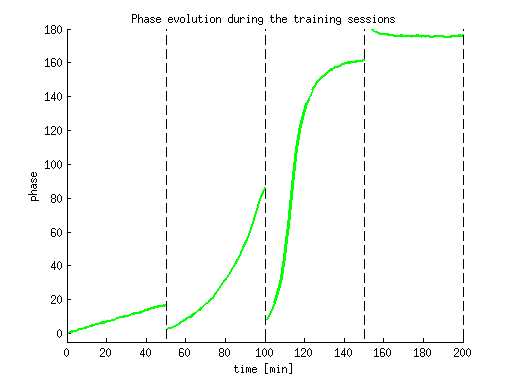
\includegraphics[scale=0.35]{images/longnoi_13.png}
    \end{figure}
  \end{columns}
\end{frame}

\begin{frame}[fragile]
  \frametitle{Reproducing Clopath's results}
  \begin{figure}
    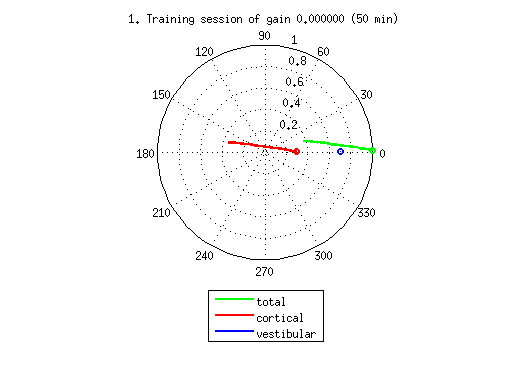
\includegraphics[scale=0.5]{images/longnoi_19.png}
    \caption{Day 1: VOR cancellation training}
  \end{figure}
\end{frame}

\begin{frame}[fragile]
  \frametitle{Reproducing Clopath's results}
  \begin{figure}
    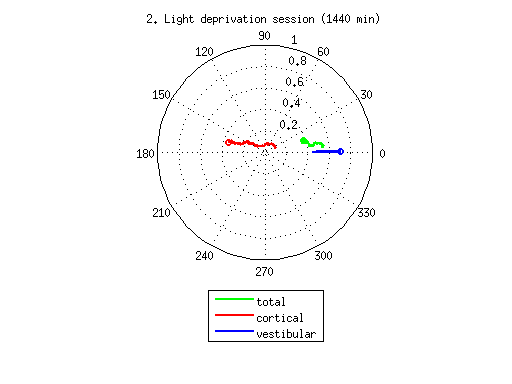
\includegraphics[scale=0.5]{images/longnoi_20.png}
    \caption{Night 1: partial extinction}
  \end{figure}
\end{frame}

\begin{frame}[fragile]
  \frametitle{Reproducing Clopath's results}
  \begin{figure}
    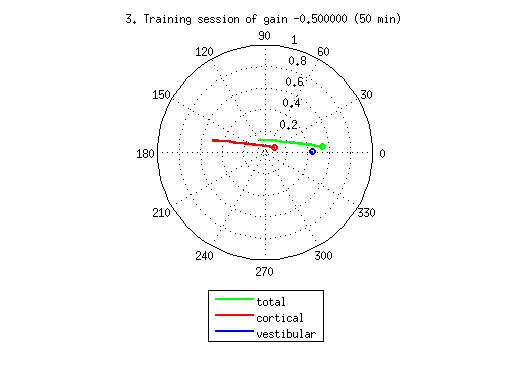
\includegraphics[scale=0.5]{images/longnoi_21.png}
    \caption{Day 2: VOR phase reversal training}
  \end{figure}
\end{frame}

\begin{frame}[fragile]
  \frametitle{Reproducing Clopath's results}
  \begin{figure}
    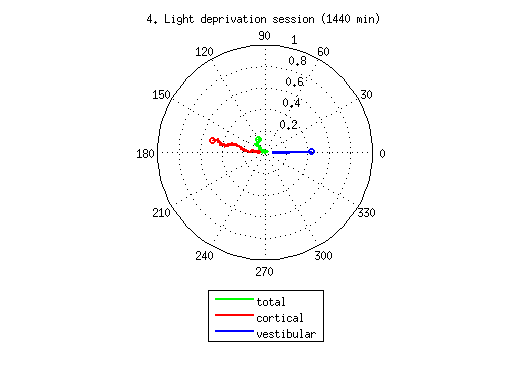
\includegraphics[scale=0.5]{images/longnoi_22.png}
    \caption{Night 2: partial extinction}
  \end{figure}
\end{frame}

\begin{frame}[fragile]
  \frametitle{What happens in the dark?}
  \begin{itemize}
    \item Cortical
      \begin{itemize}
        \item Extinguishes progressively to a baseline
      \end{itemize}
    \item Nuclear
      \begin{itemize}
        \item Continues transference from cortical memory until it arrives at a nuclear balance
      \end{itemize}
    \item Total
      \begin{itemize}
        \item Extinction and transference go in opposite directions
        \item On the dark adaptation continues consolidating until an inflextion point where extinction overtakes transference
        \item After a long period on the dark, all cortical memory is consolidated on the brainstem and cortical contribution is at its baseline
      \end{itemize}
  \end{itemize}
\end{frame}

% \begin{frame}[fragile]
%   \frametitle{What happens in the dark?}
%   \begin{columns}[onlytextwidth]
%     \column{0.5\textwidth}
%       \begin{figure}
%         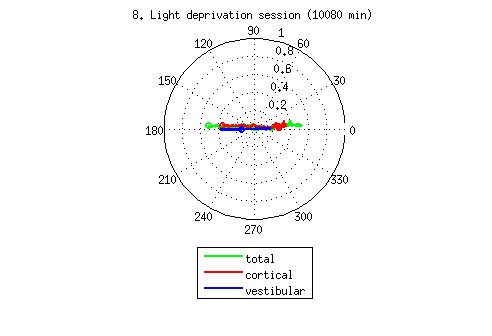
\includegraphics[scale=0.6]{images/longnoi_11.png}
%       \end{figure}
%     \column{0.5\textwidth}
%     Limitations of the model
%     \begin{itemize}
%       \item control isn't perfect
%       \item there's always some modulation on the cortical signal
%       \item nuclear transference
%     \end{itemize}
%   \end{columns}
% \end{frame}

\section{Conclusions}

\begin{frame}[fragile]
  \frametitle{Conclusions}
  \begin{itemize}
    \item NOI \textbf{explains extinction} on VOR adaptation
    \item Extinction is triggered when vestibular information is available
    \item Teaching or error signal is modulated by \textbf{cerebellar output}
    \item Savings
  \end{itemize}
\end{frame}

\begin{frame}[fragile]
  \frametitle{Conclusions}
  \begin{figure}
    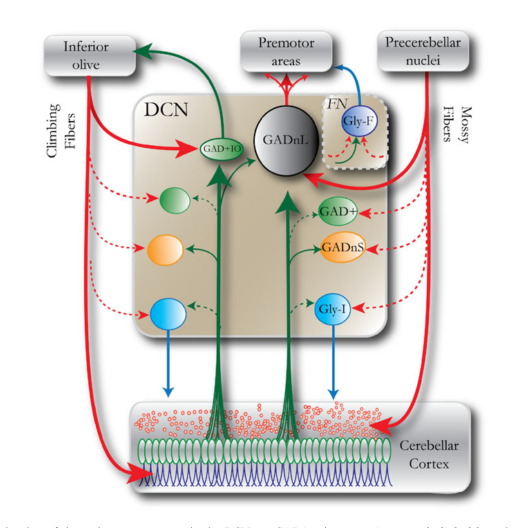
\includegraphics[scale=0.3]{images/uusisaari.png}
    \caption{GAD+IO neuron populations receive signals from cerebellar output \cite{Uusisaari2011}}
  \end{figure}
\end{frame}

\begin{frame}[fragile]
  \frametitle{Further work}
  More detailed bottom-up models
  \begin{itemize}
    \item transgenic mouse lines
    \item better electro-physiological recordings
    \item models with distributed plasticity
  \end{itemize}
\end{frame}

% \begin{frame}[fragile]
%   \fontsize{5}{8}
%   \selectfont
%   \frametitle{References}
%   \bibliography{vornoi}
% \end{frame}

\begin{frame}[fragile]
  \fontsize{5}{8}
  \selectfont
  \frametitle{References}
  \begin{thebibliography}{}

  \bibitem[Boyden et~al., 2004]{Boyden2004}
  Boyden, E.~S., Katoh, A., and Raymond, J.~L. (2004).
  \newblock {Cerebellum-dependent learning: the role of multiple plasticity
    mechanisms.}
  \newblock {\em Annu. Rev. Neurosci.}, 27:581--609.

  \bibitem[Clopath et~al., 2014]{Clopath2014}
  Clopath, C., Badura, A., {De Zeeuw}, C.~I., and Brunel, N. (2014).
  \newblock {A cerebellar learning model of vestibulo-ocular reflex adaptation in
    wild-type and mutant mice.}
  \newblock {\em J. Neurosci.}, 34(21):7203--15.

  \bibitem[Cohen et~al., 2004]{Cohen2004}
  Cohen, M.~R., Meissner, G.~W., Schafer, R.~J., and Raymond, J.~L. (2004).
  \newblock {Reversal of motor learning in the vestibulo-ocular reflex in the
    absence of visual input.}
  \newblock {\em Learn. Mem.}, 11(5):559--565.

  \bibitem[Emken et~al., 2007]{Emken2007}
  Emken, J.~L., Benitez, R., Sideris, A., Bobrow, J.~E., and Reinkensmeyer, D.~J.
    (2007).
  \newblock {Motor adaptation as a greedy optimization of error and effort.}
  \newblock {\em J. Neurophysiol.}, 97(6):3997--4006.

  \bibitem[Gao et~al., 2012]{Gao2012a}
  Gao, Z., van Beugen, B.~J., and {De Zeeuw}, C.~I. (2012).
  \newblock {Distributed synergistic plasticity and cerebellar learning.}
  \newblock {\em Nat. Rev. Neurosci.}, 13(9):619--35.

  \bibitem[Herreros and Verschure, 2013]{Herreros2013b}
  Herreros, I. and Verschure, P. F. M.~J. (2013).
  \newblock {Nucleo-olivary inhibition balances the interaction between the
    reactive and adaptive layers in motor control.}
  \newblock {\em Neural Netw.}, 47:64--71.

  \bibitem[Medina et~al., 2002]{Medina2002}
  Medina, J.~F., Nores, W.~L., and Mauk, M.~D. (2002).
  \newblock {Inhibition of climbing fibres is a signal for the extinction of
    conditioned eyelid responses.}
  \newblock {\em Nature}, 416(6878):330--333.

  \end{thebibliography}
\end{frame}

\begin{frame}[fragile]
  \fontsize{5}{8}
  \selectfont
  \frametitle{References}
  \begin{thebibliography}{}

  \bibitem[Schonewille et~al., 2010]{Schonewille2010}
  Schonewille, M., Belmeguenai, a., Koekkoek, S.~K., Houtman, S.~H., Boele,
    H.~J., van Beugen, B.~J., Gao, Z., Badura, a., Ohtsuki, G., Amerika, W.~E.,
    Hosy, E., Hoebeek, F.~E., Elgersma, Y., Hansel, C., and {De Zeeuw}, C.~I.
    (2010).
  \newblock {Purkinje cell-specific knockout of the protein phosphatase PP2B
    impairs potentiation and cerebellar motor learning.}
  \newblock {\em Neuron}, 67(4):618--28.

  \bibitem[Uusisaari and Kn\"{o}pfel, 2011]{Uusisaari2011}
  Uusisaari, M. and Kn\"{o}pfel, T. (2011).
  \newblock {Functional classification of neurons in the mouse lateral Cerebellar
    Nuclei}.
  \newblock {\em Cerebellum}, 10(4):637--646.

  \bibitem[Yamazaki et~al., 2015]{Yamazaki2015}
  Yamazaki, T., Nagao, S., Lennon, W., and Tanaka, S. (2015).
  \newblock {Modeling memory consolidation during posttraining periods in
    cerebellovestibular learning}.
  \newblock {\em Proc. Natl. Acad. Sci.}, 112(11):201413798.

  \end{thebibliography}
\end{frame}

\plain{Thank you}

\end{document}
